\documentclass[]{article}

\usepackage{siunitx}
\usepackage{amsmath}
\usepackage{amssymb}
\usepackage{wasysym}
\usepackage{graphicx}
\usepackage{wrapfig}
\usepackage{algorithm}
\newcommand{\abs}[1]{\left|#1\right|}
\newcommand{\ReF}{\operatorname{Re}}
\newcommand{\Lap}{\mathcal{L}}
\newcommand{\B}[1]{\boldsymbol{#1}}
\newcommand{\p}{\text{proj}}
\newcommand{\R}{\mathbb{R}}
\newcommand{\Dv}[1]{\mathcal{R}_{\B{#1}}}
\newcommand{\Q}{\mathbb{Q}}
\newcommand{\Z}{\mathbb{Z}}
\newcommand{\I}[1]{#1^\text{int}}
\newcommand{\bnd}[1]{\partial #1}
\newcommand{\mx}[1]{\text{max}(#1)}
\newcommand{\mn}[1]{\text{min}(#1)}
\newcommand{\ceil}[1]{\lceil #1 \rceil}
\newcommand{\pd}{\partial}
\newcommand{\eval}[3]{\left.#1\right|_#2^#3}
\newcommand{\del}[2]{\pd_{#2} #1}
\newcommand{\delH}[3]{\pd^{#1}_{#3} #2}
\newcommand{\Int}[2]{\int\limits_{#1}^{#2}}
\newcommand{\IInt}{\int\!\!\!\!\int}
\newcommand{\IIInt}{\int\!\!\!\!\int\!\!\!\!\int}
\newcommand{\Sum}[2]{\sum\limits_{#1}^{#2}}
\newcommand{\Uni}[2]{\bigcup\limits_{#1}^{#2}}
\newcommand{\VA}[3]{\left(\begin{array}{c}
#1\\
#2\\
#3
\end{array}\right)}
\newcommand{\tab}{\hspace*{.25in}}
\newcommand{\qed}{\hfill\square }
\newcommand{\A}{\text{A}}
\newcommand{\uth}{^{\text{th}}}
\newcommand{\Hline}{\noindent\rule[0.5ex]{\linewidth}{.5pt}}
\newcommand{\txtfn}[2]{\text{#1}\left(#2\right)}
\graphicspath{c:/users/joseph/documents/"MATH 336"/"Term Paper"}


\usepackage[T1]{fontenc}
\usepackage[latin9]{inputenc}
\usepackage{amsmath}
\usepackage{amsthm}
\usepackage{amssymb}
%\usepackage{esint}

% matrix environment for vectors or matrices where elements are centered
\newenvironment{mat}{\left[\begin{array}{ccccccccccccccc}}{\end{array}\right]}
\newcommand\bcm{\begin{mat}}
\newcommand\ecm{\end{mat}}

% matrix environment for vectors or matrices where elements are right justifvied
\newenvironment{rmat}{\left[\begin{array}{rrrrrrrrrrrrr}}{\end{array}\right]}
\newcommand\brm{\begin{rmat}}
\newcommand\erm{\end{rmat}}



\usepackage{geometry}                % See geometry.pdf to learn the layout options. There are lots.
\geometry{letterpaper}                   % ... or a4paper or a5paper or ... 
%\geometry{landscape}                % Activate for for rotated page geometry
%\usepackage[parfill]{parskip}    % Activate to begin paragraphs with an empty line rather than an indent

\usepackage{graphicx}
\usepackage{amssymb}
\usepackage[all]{xy}
\usepackage{epstopdf}
\DeclareGraphicsRule{.tif}{png}{.png}{`convert #1 `dirname #1`/`basename #1 .tif`.png}
\theoremstyle{plain}
\newtheorem{thm}{\protect\theoremname}
  \theoremstyle{definition}
  \newtheorem{xca}[thm]{\protect\exercisename}
  
\usepackage{setspace}
%\doublespacing
\onehalfspacing

\newcommand{\algostart}[1]{\Hline\\\textbf{#1}\\\Hline\\}


%TODO: change title to:
\title{Hessian-Free Optimization and its applications to Neural Networks}
%\title{Using Neural Networks to for Optical Character Recognition}

\author{Joseph Christianson}

\begin{document}
\maketitle

\begin{abstract}
Neural Networks are a simple model of biological cognitive processes. In this paper we introduce how the Neural Network operates, summarizing key sections of A.C.C. Coolen's large introductory paper. We examine their biological motivations, how they process data, and the default training method of gradient descent and backpropogation. We then analyze an optimization to the traditional structure provided by James Martens. His technique improves upon gradient descent by employing second order derivatives and he introduces a numerically stable way to calculate them. 
\end{abstract}

\section{Biological Motivation}

Neural Networks are an abstraction of the way we understand brains process information. Brains are composed of huge networks of individual neurons. Brains neurons act as individual processors. They sit in a ion rich fluid that causes there to be an electrical gradient between the inside of the neuron cell and the outside. When a neuron is electrically stimulated, pumps open and the fluid enters the cell. This causes a generation of electrical current which spreads along the membrane. This action is called firing. In this way a signal can propagate from neuron to neuron.

Neurons are connected by dendrites, synapses, and an axon. Each neuron only as one axon. When a neuron fires, the signal travels down its membrane. Dendrites are thread-like membranes that bring signals to a neuron. They are connected to axons of other neurons via synapses. Synapses have a synaptic cleft, were the cell membranes interface without being contiguous. Each synapse stores a certain amount of positive and negatively charged fluid called neurotransmitter. When a signal reaches a synapse its neurotransmitter is released. Positively charged neurotransmitter provides an excitatory signal, while negatively charged provides an inhibitory one. The amount of neurotransmitter released modulates the strength of the signal passed along to the dendrite, and so is called a synaptic weight.

Overall brains are simply huge networks of these neurons. The network structure and synaptic weights store the "program" of the brain. This includes both behavior and memory. The brain continuously adapts by adjusting the weights and connections present. Neurons themselves are somewhat unreliable as they fire as a result of input, but also sometimes spontaneously. This results in a high degree of redundancy in structure and makes the brain more resilient and adaptable. 
 
In drawing a comparison to digital computers, rather than having a few deterministic, powerful processors, a brain is a massively parallel network of low power stochastic processors. Additionally, where as computers generally keep program instructions separate from memory, brains do not differentiate.

\section{Modelling}
With the above description in mind, we now tackle creating a simple model of neural activity. Suppose we have $ N $ neurons. Then at time $ t_0 $ we express the input signal to the $ i $th neuron as: 
\[ \text{input}_i = w_1S_1 + ... + w_NS_N,\] 
where $ w_j $ is the synaptic weight connecting the $ j $th neuron to the $ i $th neuron. $ S_j $ is the signal generated by the $ j $th neuron. If the $ i $th neuron has some signal threshold, $ \theta_i $ over which it fires then we can create a function for activation:
\[ S_i(t+1) = \left\{\begin{array}{lcr}
1 &:& w_1S_1(t) + ... + w_NS_N > \theta_i\\
0 &:& w_1S_1 + ... + w_NS_N \leq \theta_i
\end{array}\right. \]
The final step is to decide if we apply this function to all neurons at once in a single time step, to randomly choose neurons to update, or to update single neurons in a set sequence. A neural network then is just a set of binary values, updated by this rule.

\section{Computability} 
From this simple model we can glean a powerful piece of information. Neural networks as we have defined them are universal computing machines. Coolen's proof for this is to show that neural networks can encode the logical \texttt{AND}, \texttt{OR}, and \texttt{NOT}.

\begin{figure}[h]
\centering
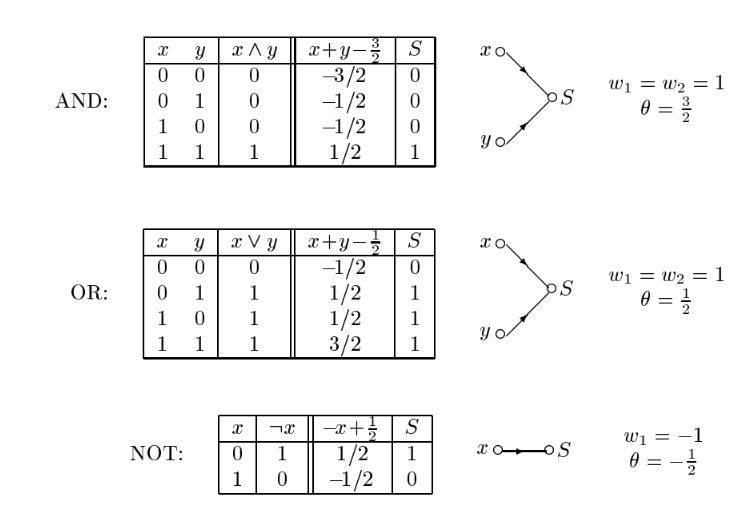
\includegraphics[scale=1]{CoolenProof.jpg}
\end{figure}

\texttt{AND} becomes two input dendrites with synapses of weight $ 1 $, connected to a single neuron with threshold $ \theta = 3/2 $.
\texttt{OR} becomes two input dendrites with synapses of weight $ 1 $, connected to a single neuron with threshold $ \theta = 1/2 $.
\texttt{AND} becomes one input dendrite with synapse of weight $ -1 $, connected to a single neuron with threshold $ \theta = -1/2 $.

\section{Architecture}
There are many ways to organize neurons into neural networks with each being suited to different tasks. We will focus on one called ``feed forward.'' Here neurons are organized into layers. Each neuron in a layer receives input from every neuron in the layer before it, and outputs to every neuron in the layer after. Neurons are not connected to other neurons in their layer, nor to layers beyond those immediately adjacent. The neural network can then be operated by updating every neuron in a layer simultaneously, and the layers sequentially. 

Successfully operating a feed forward network then becomes a matter of figuring out which weights and thresholds produce the desired result. This process is called learning because the network is physically storing information. Learning methods can be divided into two categories, supervised and unsupervised. We will focus on the former. 

Supervised learning has three main steps. First, acquire a dataset of questions and answers in the form of bit arrays. Then, set the initial signals of the first layer, the input layer, to the bit array of a question. Perform the neural network operation and observe the difference between the output (the signals of the last layer) and the given answer. Then by some rule we adjust the weights to reduce future error. This process repeats until the network does well enough on all the questions. 

Coolen presents a basic example of this in a network with a single neuron.
\begin{figure}[h]
\centering
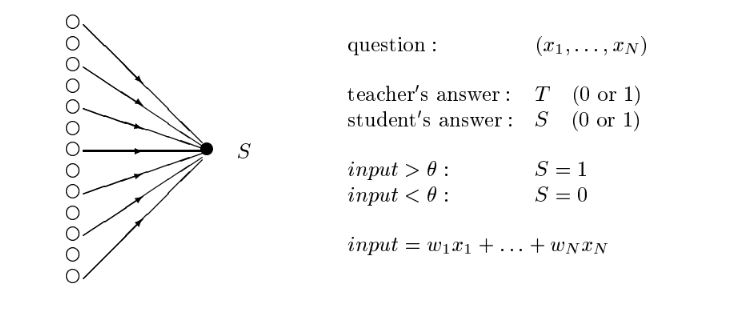
\includegraphics[scale=0.70]{CoolenPerceptron.jpg}
\end{figure}

Given the above definitions, the learning rule is as follows: for a given question $ (x_1,..., x_N) $ compare $ S = S(x_1,...,x_N ) $ and $ T = T(x_1,...,x_N ) $. Proceed as follows:
\begin{table}[h]
\begin{tabular}{ll}
if $ S=T $: & do nothing\\
if $ S = 1 $, $ T = 0 $:& Set $ w_i = w_i - x_i $ and $ \theta = \theta + 1 $\\
if $ S = 0 $, $ T = 1 $:& Set $ w_i = w_i + x_i $ and $ \theta = \theta - 1 $\\
\end{tabular}
\end{table}
Such a neuron with a learning rule is called a perceptron. 
Coolen asserts that this rule comes with a proof of convergence. Formally he states:

\textit{If values for the parameters $ \{w_l\} $ and $ \theta $ exists, such that $ S = T $ for each
question $ (x_1,...,x_N ) $, then the perceptron learning rule will find these,
or equivalent ones, in a finite number of modification steps.}

His proof follows:

Assume $ \Omega $ is a finite and discrete set of questions. Rather than keeping track of the threshold separately, we let $ x_0 = -1 $, and say $ w_0 = \theta $. Now we can establish a weight vector $ \B{w} = (w_0, w_1, ..., w_N) $ and a question vector as $ \B{x} = (x_0, x_1, ..., x_N) $. Operation now simply becomes:
\[ \B{w}\cdot \B{x} > 0 \to S = 1,\qquad \B{w}\cdot \B{x} \leq 0 \to S = 0\]
and the learning rule becomes
\[ \B{w} = \B{w} + [T(\B{x}) - S(\B{x})]\B{x} \]
We have assumed that some weight vector $ \B{w}' $ exists such that 
\[T(\B{x}) = 1\implies\B{w}'\cdot \B{x} > 0,\qquad T(\B{x}) = 0\implies\B{w}'\cdot \B{x} \leq 0\]
Now define $ X = \max\{\abs{\B{x}}:\B{x}\in\Omega\} > 0 $ and $ \delta = \min\{\abs{\B{w}'\cdot\B{x}}:\B{x}\in\Omega\} > 0 $. Then for all $ \B{x}\in\Omega,  \abs{\B{x}}\leq X $ and $ \abs{\B{w}'\cdot\B{x}} \geq \delta $. Next we examine the modification step $ w\to w_1 $. We know $ S = 1-T $, otherwise there would be no modification. We examine two quantities:
\[ \B{w}_1\cdot \B{w}' = \B{w}\cdot \B{w}' + [2T(\B{x}) - 1]\B{x}\cdot \B{w}' \qquad 
\abs{\B{w}_1}^2 = \abs{\B{w}}^2 + 2[2T(\B{x}) - 1]\B{x}\cdot\B{w} + [2T(\B{x}) - 1]^2\abs{\B{x}}^2\]
If $ \B{w}'\cdot\B{x} \leq 0 $ then $ 2T(\B{x}) - 1 = -1 $ and if $ \B{w}'\B{x} > 0, $ and that therefore $ [2T(\B{x}) - 1]\B{x}\cdot\B{x}<0 $, so the above quantities simplify to:
\[ \B{w}_1\cdot \B{w}' = \B{w}\cdot \B{w}' + \abs{\B{x}\cdot \B{w}'} \geq \B{w}\cdot\B{w}'+\delta\qquad 
\abs{\B{w_1}}^2 < \abs{\B{w}}^2 + \abs{\B{x}}^2 \leq \abs{\B{w}}^2 + X^2\]
After $ n $ iterations, we find:
\[ \B{w}_n\cdot \B{w}' 
\geq \B{w}\cdot\B{w}'+n\delta\qquad 
\abs{\B{w_n}}^2 \leq \abs{\B{w}}^2 + nX^2\]
Yields:
\[ \frac{\B{w}_n\cdot\B{w}'}{\abs{\B{w}'}\abs{\B{w}_n}} 
\geq
\frac{\B{w}\cdot\B{w}'+n\delta}{\abs{\B{w}'}\sqrt{\abs{\B{w}}^2 + nX^2}}
\implies
\lim\limits_{n\to\infty}\frac{1}{\sqrt{n}}\frac{\B{w}_n\cdot\B{w}'}{\abs{\B{w}'}\abs{\B{w}_n}}
\geq
\frac{\delta}{\abs{\B{w}'}X} > 0
\]
Therefore the number of iterations must be bounded, other this is a contradiction of the Schwarz inequality $ \abs{\B{w}\cdot\B{w}'}\leq \abs{\B{w}}\abs{\B{w}'}$. If no more modifications can be made then $ S(\B{x}) = T(\B{x}) $ for every $ \B{x}\in\Omega $. $ \qed $

This theorem relied on the assumption that a solution exists. The binary operation \texttt{XOR} is a simple example that not every operation $ \{0,1\}^N\to\{0,1\} $ is computable by a single perceptron. The requirement is that
\[ \texttt{XOR}(x_1, x_2) = 1 \implies w_1x_1 + w_2x_2 > \theta
\qquad \text{and}\qquad
\texttt{XOR}(x_1, x_2) = 0 \implies w_1x_1 + w_2x_2 \leq \theta\]
The truth table:
\begin{figure}[h]
\centering
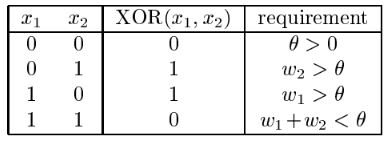
\includegraphics[scale=01]{CoolenXORtable.jpg}
\end{figure}
show that the requirements are impossible. 

The solution to this problem is coupling perceptron's together, to form networks. Networks can tackle binary or real valued problems. Coolen provides a proof of computability for binary transformations. Regular (usually meaning bounded domain), real functions are modeled by using a real valued activation function, rather than the step function we previously introduced. These functions are continuous, non-decreasing, and bounded. Common choices are $ \tanh(s) $ or $ \txtfn{erf}{s} $, where s is the dot product of signals and weights.

%todo: roughly here comment on switching to nieslsen for a description of training large networks

%Coolen's example is a basic multi-layer network. It has an input layer, single hidden layer, and single perceptron for the output. Thus the output (the student's answer) is \[ S(x_1, x_2, ..., x_n) = f(w_1y_1+...+w_ky_k-\theta), where y_l(x_1, ..., x_n) = f(w_{l1}+...+w_{ln}x_n-\theta_l) \]. The thresholds can be eliminated with dummy variables. 

Now we need to construct a learning rule. We quantify the error as:
\[ E = \frac{1}{2}\sum\limits_{\B{x}\in\Omega}p(\B{x})\left[T(\B{x}) - S(\B{x})\right]^2, \] 
where $ p(\B{x}) $ is the proportion of the sample data that is question $ \B{x} $, assuming no duplicates, this is $ 1/N $, $ \Omega $ is the set of questions, and $ T(\B{x}) $ and $ S(\B{x}) $
are the teacher and student's answers respectively. We can minimize this using gradient descent. Nielsen has a better description of how this process actually works, so we'll follow his lead for the moment. 

We seek to minimize the error using the gradient descent method. This means we visualize all the possible weights as a high dimensional space, then taking the gradient of the cost function will point us in the optimum direction to maximize the cost function. We therefore choose a small positive scalar $ \eta $ and define an update step to be
\[ w_{i+1} = w_i - \eta\nabla E. \]
We can then iterate on the weights as a whole until the error is small enough. 

Computing the gradient of the error function can be quite difficult. The common approach is to use the backpropogation algorithm, which Coolen does not detail. For an explanation we turn to Michael Nielsen's book on deep learning.
\subsection{Nielsen's Description of Backpropogation}
Notation is difficult to keep track, so we will introduce Nielsen's carefully. He denotes the weight connecting the $ k\uth $ neuron in the $ (l-1)\uth $ layer to the $ j\uth $ neuron in the $ l\uth $ layer with:
$ w^l_{jk} $. Each neuron's bias is denoted by $ b_j^l $ and the activation is $ a_j^l $ where $ l $ and $ j $ are still layer and neuron number respectively. Using these definitions we can write the activation of any neuron as
\[ a^l_j = \sigma\left(\sum\limits_\textsl{}{k}w^l_{jk}a^{l-1}_k + b_j^l\right) \]
where $ \sigma $ is the chosen activation function (Nielsen, eq 23). We adapt this 
notation to write an expression for all of the activations by forming matrices and 
vectors of like terms. Each layer has an associated weight matrix $ w^l $, where $ 
w^l_{jk} $ is the $ k\uth $ element in the $ j\uth $ row. Likewise, we can form bias 
and activation vectors $ b^l $ and $ a^l $ respectively. Now we can describe the 
activation of an entire layer at once 
\[ a^l = \sigma(w^la^{l-1}+b^l). \]
In this form sigma is vectorized so it maps from $ \R^n $ to $ \R^n $. A final note on notation, $ z^l = w^la^{l-1}+b^l $ is called the weighted input. 

Backpropagation is an efficient and clear way of computing the partial derivatives of the error function, which we can then feed into gradient descent. Recall we have written the error function as 
\[ E = \frac{1}{2n}\sum\limits_{\B{x}\in\Omega}\left[T(\B{x}) - a^L(\B{x})\right]^2, \] 
where $ n $ is the number of questions in some set $ \Omega $, $ T(\B{x}) $ is the correct answer, $ L $ is the number of layers in the network and $ a^L(\B{x}) $ is the activation of the final layer given $ \B{x} $ as input to the network.

The way backpropagation works is by computing the partial derivatives $ \pd E/\pd w_{jk}^l $ and $ \pd E/\pd b_{j}^l $ for individual training samples and then average over the whole set. 

Let $ \delta_j^l $ be the individual error for each neuron, defined as
\[ \delta_j^l = \frac{\pd E}{\pd z^l_j} \]

Backpropogation can be decomposed into four fundamental equations:
\[ \delta^L_j = \frac{\pd E}{\pd a^L_j}\sigma'\left(z^L_j\right) \qquad \text{or in matrix form}\qquad \delta^L = \nabla_{a^L}E\odot\sigma'\left(z^L\right)\]
Using the square error function defined above, we can further simplify this to:
\[ \delta^L = (a^L - T(\B{x}))\odot\sigma'\left(z^L\right). \]

Next we formulate an expression for the error $ \delta^l $ in terms of the error $ \delta^{l+1} $. This is where the name backpropogation starts to make sense, because such as equation will allow us to move backwards through the network. Such an equation is
\[ \delta^l = ((w^{l+1})^T \delta^{l+1})\odot\sigma'(z^l). \]

Now that we have the tools to compute the error for any neuron at any layer, we want to compute the partial derivatives.
\[ \frac{\pd E}{\pd b_j^l} = \delta_j^l \qquad \text{ and }\qquad \frac{\pd E}{\pd w_{jk}^l} = a_k^{l-1}\delta_j^l \]
We can now proceed using the gradient descent method previously described. Backpropogation simply evaluates the gradient for us. 


%\algostart{Algorithm 1 - Gradient Descent}
%\textbf{Inputs}: $ \B{b}, A, \B{x}_0 $\\
%$ \B{r}_0 \leftarrow \B{b} $\\
%$ \B{y}_0 \leftarrow \B{r}_0 $\\
%%$ \B{p}_0 \leftarrow -\B{y}_0 $\\
%$ i \leftarrow 0 $\\
%\textbf{while} termination condition is false \textbf{do}\\
%\tab$ \alpha_i \leftarrow \displaystyle\frac{\abs{\B{r}_i}^2}{\B{y}_i^TA\B{y}_i} $\\
%\tab$ \B{x}_{i+1} \leftarrow \B{x_i} + \alpha_i\B{y}_i$\\
%\tab$ \B{r}_{i+1} \leftarrow \B{r}_i + \alpha_iA\B{y}_i $\\
%%\tab$ \B{y}_{i+1} \leftarrow $ solution of $ P\B{y}_i = \B{r}_{i+1}$\\
%\tab$ \beta_{i+1}\leftarrow\displaystyle\frac{\abs{\B{r}_{i+1}}^2}{\abs{\B{r}_{i}}^2} $\\
%\tab$ \B{y}_{i+1} \leftarrow \B{r}_{i+1}+\beta_{i+1}\B{y}_i $
%\tab$ i\leftarrow i+1 $\\
%\textbf{end while}\\
%\textbf{output:} $ \B{x}_i $\\
%\Hline



\section{Better Training through Hessian Free Optimization}

Gradient descent scales well laterally, meaning it works well for layers with many neurons, however it does not work on deep nets that have many layers. It also exhibits issues with functions that have pathological curvature. These are functions where the direction of steepest descent is not a good approximation of the direction to a local minimum. An example of such pathological curvature is the Rosenbrock function. This function can be pictured as a horseshoe shaped valley. The minimum is located at the apex of the horseshoe. The walls of the valley are steep, but the floor only slopes gradually. The gradient descent algorithm does not perform well on this function because the direction of steepest descent points across the horseshoe rather than along it. This causes each iteration of the gradient descent to bounce back and forth across the horseshoe, only slowly converging to the true minimum. 

\begin{figure}['h']
\centering
\includegraphics[scale=0.25]{rosenbrock.jpg}
\caption{The Rosenbrock Function}
\end{figure}

A method of combating such issues in minimization is to employ a second-order technique. Gradient descent is a first-order technique because it only relies on the first derivatives, in the form of the gradient, of the function. Second-order techniques on the other hand, rely on second-order derivatives which provide information about the curvature. 

The canonical example of a second order scheme is Newton's Method, which relies on the fact that for $ \B{\delta} $ where $ \abs{\B{\delta} } $ is small:
\[ f(\B{x}_k+\B{\delta}) \approx M_k(\B{\delta} ) = f(\B{x}_k) + \nabla f(\B{x}_k)\cdot\B{\delta} + \frac{1}{2}\B{\delta}\cdot H(\B{x}_k)\B{\delta}.\]
Where $ \nabla f(\B{x}) $ is the gradient and $ H(\B{x}) $ is the Hessian matrix. We then try to minimize $ M(\B{\delta}) $ iteratively. For a given $ \B{\delta}_k $, we compute that $ \B{\delta}_{k+1} = \B{\delta}_k + \alpha_k\B{\delta}_k^* $, where $ \B{\delta}_k^* $ minimizes $ M_k(\B{\delta}) $ and $ \alpha_k\in[0,1] $ is the step length. If $ H(\B{x_k}) $ is positive definite, then $ M_k(\delta) $ will be bounded below. This guarantees that $ \B{\delta}_k^* $ exists, and it can be shown that $ \B{\delta}_k^* $ is given by
\[ \B{\delta}_k^* = -H(\B{x}_k)^{-1}\nabla f(\B{x}_k) \text{\qquad or equivalently by solving\qquad} H(\B{x}_k)\B{\delta}_k^* = -\nabla f(\B{x}_k) \]

The issue with this method is that even computing, must less inverting, the Hessian Matrix is prohibitively expensive for machine learning applications. Martens introduces two approximations into this method that allow for significant increases in efficiency while maintaining accuracy. The first is utilizing the conjugate gradient algorithm to minimize $ M_k(\B{\delta}) $. The conjugate gradient is a powerful method in its own right, but a chief advantage in this context, is that it allows us to never form the Hessian matrix directly. This is where the Hessian Free name comes from. The second, is a numerically stable method of computing the Hessian.

\subsection{Conjugate Gradient}
Here we provide an brief explanation and pseudo-code for the conjugate gradient algorithm. Conjugate gradient finds a solution to the linear system $ A\B{x} = b $, by finding a minimizer to the quadratic function $ \phi:\R^n \to \R $. $ \phi(\B{x}) $ is  defined as $ \phi(\B{x}) = 1/2\B{x}^TA\B{x}-b^T\B{x} $. Below we illustrate the process. 
%\newpage
\algostart{Conjugate Gradient}
\textbf{Inputs}: $ \B{b}, A, \B{x}_0 $\\
$ \B{r}_0 \leftarrow \B{b} $\\
$ \B{y}_0 \leftarrow \B{r}_0 $\\
%$ \B{p}_0 \leftarrow -\B{y}_0 $\\
$ i \leftarrow 0 $\\
\textbf{while} termination condition is false \textbf{do}\\
\tab$ \alpha_i \leftarrow \displaystyle\frac{\abs{\B{r}_i}^2}{\B{y}_i^TA\B{y}_i} $\\
\tab$ \B{x}_{i+1} \leftarrow \B{x_i} + \alpha_i\B{y}_i$\\
\tab$ \B{r}_{i+1} \leftarrow \B{r}_i + \alpha_iA\B{y}_i $\\
%\tab$ \B{y}_{i+1} \leftarrow $ solution of $ P\B{y}_i = \B{r}_{i+1}$\\
\tab$ \beta_{i+1}\leftarrow\displaystyle\frac{\abs{\B{r}_{i+1}}^2}{\abs{\B{r}_{i}}^2} $\\
\tab$ \B{y}_{i+1} \leftarrow \B{r}_{i+1}+\beta_{i+1}\B{y}_i $
\tab$ i\leftarrow i+1 $\\
\textbf{end while}\\
\textbf{output:} $ \B{x}_i $\\
\Hline
%\algostart{Algorithm 1 - Conjugate Gradient}
%\textbf{Inputs}: $ \B{b}, A, \B{x}_0 $\\
%$ \B{r}_0 \leftarrow A\B{x}_0 - \B{b} $\\
%$ \B{y}_0 \leftarrow -\B{r}_0 $\\
%%$ \B{p}_0 \leftarrow -\B{y}_0 $\\
%$ i \leftarrow 0 $\\
%\textbf{while} termination condition is false \textbf{do}\\
%\tab$ \alpha_i \leftarrow \displaystyle\frac{\B{r}_i^T\B{y}_i}{\B{y}_i^TA\B{y}_i} $\\
%\tab$ \B{x}_{i+1} \leftarrow \B{x_i} + \alpha_i\B{y}_i$\\
%\tab$ \B{r}_{i+1} \leftarrow \B{r}_i + \alpha_iA\B{y}_i $\\
%%\tab$ \B{y}_{i+1} \leftarrow $ solution of $ P\B{y}_i = \B{r}_{i+1}$\\
%\tab$ \beta_{i+1}\leftarrow\displaystyle\frac{\B{r}^T_{i+1}\B{y}_{i+1}}{\B{r}^T_{i}\B{y}_{i}} $\\
%\tab$ \B{y}_{i+1} \leftarrow -\B{y}_{i+1}+\beta_{i+1}\B{y}_i $
%\tab$ i\leftarrow i+1 $\\
%\textbf{end while}\\
%\textbf{output:} $ \B{x}_i $\\
%\Hline

Marten's version is slightly more complicated, because he includes pre-conditioning. Pre-conditioning maps the entire process to a more favorable coordinate system, which allows for faster convergence. I do not discuss it in this paper, so I have omitted it from the algorithm.

The termination condition of the iteration requires its own discussion. One might propose conditions such as $ \abs{A\B{x} - \B{b}}_2 < \epsilon $. While this is in line with the goal of the iteration, it does not reflect what the method is actually doing. Because the conjugate gradient is minimizing $ \phi(\B{x}) = 1/2\B{x}^TA\B{x}-b^T\B{x} $, it is not guaranteed that $ \abs{A\B{x} - \B{b}}_2 $ will steadily decrease, even though they both have the same minimizer. Instead Marten's proposes a convergence condition based on the Cauchy condition for convergence. He prescribes terminating the loop if for:
\[ i > k \text{\quad and\quad} \phi(\B{x}_i) < 0 \text{\quad and\quad} \frac{\phi(\B{x}_i) - \phi(\B{x}_{i-k})}{\phi(\B{x}_i)}
< k\epsilon \]
where $ k $ is how many iterations in the past we look, an varies over time. Marten's choose to set $ k = \max(10, 0.1i) $\footnote{Being in the complex analysis mindset, this confused me for longer than it should have.}. 

Martens has several further optimizations for the conjugate gradient, but the final one that we will mention here is sharing information across iterations. This is accomplished by clever choice of the $ \B{x}_0 $ parameter. Rather follow the standard practice of setting $ \B{x}_0 = (0,...,0)^T $, we set it to the final value for $ y_i $ from the previous time the conjugate gradient was run. Call this value $ y_{n-1} $. Martens reports experimental gains from this and hypothesizes that while $ \phi(y_{n-1}) $ may not be close to 0, the directions of $ y_{n-1} $ most responsible for the increase will be minimized first by the conjugate gradient, while preserving the most progress towards the minimum.


\subsection{Computing the Hessian}
The trick to avoid forming the Hessian completely is to form the product $ H(\B{x})\B{\delta} $ directly. We can do this by recognizing that the Hessian is just the Jacobian of the gradient, so $ H(\B{x})\B{\delta} $ is the directional derivative of the gradient $ \nabla f(\B{x}) $ in the $ \B{v} $ direction. This gives us that
\[ H(\B{x})\B{\delta} = \lim\limits_{\epsilon\to0}\frac{\nabla f(\B{x} + \epsilon\B{\delta}) - \nabla f(\B{x})}{\epsilon}. \]
This is the intuition we will employ going forward, however, computing this limit as a finite difference is not numerically stable. 

To solve this problem Martens instead utilizes a technique called ``forward differentiation.'' We denote the direction derivative operation of the gradient by
\[ \Dv{\delta} \{\nabla f(\B{x})\} = H(\B{x})\B{\delta} = \lim\limits_{\epsilon\to0}\frac{\nabla f(\B{x} + \epsilon\B{\delta}) - \nabla f(\B{x})}{\epsilon}\]

First thing to note is that even though these are special kinds of derivatives, they still obey all the usual rules of derivatives.
\[ \Dv{v}(x+y) = \Dv{v}x + \Dv{v}y \]
\[ \Dv{v}(xy) = \left(\Dv{v}x\right)y + \left(\Dv{v}y\right)x \]
\[ \Dv{v}(\gamma(x)) = \left(\Dv{v}x\right)J_\gamma(x),  \text{\qquad where $ J_\gamma(x) $ is the Jacobian of $ \gamma $}  \]

In the same way that we had to use backpropogation to compute the gradient of the error function, we must break the computation of $ H(\B{x})\B{\delta} = \Dv{\delta}\left(\nabla f(\B{x})\right) $ into simpler parts to compute it. Here we follow Pearlmutter's explanation because it more closely follows Nielsen's description of the backpropogation method. Note, that for slightly more concise notation we let $ R = \Dv{\delta} $  
%
%\[ R(x_i) = \sum\limits_{j}\left(w_{ji}R(y_j) + v_{ji}y_j\right)
%	\implies
%		R(z^l_i) = \sum\limits_{j}\left(w_{ji}^lR(a^{l-1}_j) + v_{ji}y_j\right)  \]
%\[ R(y_i) = R(x_i)\sigma_i'(x_i)\]
%\[ R\left(\displaystyle\frac{\pd E}{\pd y_i}\right) = e_i'(y_i)R(y_i) + \sum\limits_{j}\left(
%w_{ij}R\left(\displaystyle\frac{\pd E}{\pd x_j}\right) + v_{ij}\displaystyle\frac{\pd E}{\pd x_j}\right) \]
%\[ R\left(\displaystyle\frac{\pd E}{\pd x_i}\right) = \sigma_i'(x_i)R\left(\displaystyle\frac{\pd E}{\pd y_i}\right) + R(x_i)\sigma''_i(x_i)\frac{\pd E}{\pd y_i}\]
%\[ R\left(\displaystyle\frac{\pd E}{\pd w_{ij}}\right) = y_iR\left(\displaystyle\frac{\pd E}{\pd x_j}\right) + R(y_i)\displaystyle\frac{\pd E}{\pd x_j}\]
%$ R(\pd E/\pd w_{ij}) $ is the components of $ R(\nabla E) = H(\B{x})\B{\delta} $, so we have computed what we want.
%
%%We know that $ z^l_i = w^l_{jk}a^{l-1}_k + b_j^l $, so 
%%$ R{z^l_i} = \sum\limits_{j}\left(w\right) $
%
%%This results in the following algorithm. Note, that for slightly more concise notation we let $ R = \Dv{\delta} $
%%
\algostart{Computing $ H(\B{x})\B{\delta} $}
\textbf{input}: $ \B{\delta} $ unpacked as $ (RW_1, ..., RW_L, Rb_1, ... ,Rb_L) $\\
$ Ra_0\leftarrow 0 $\\
\textbf{for $ i $ from $ 1 $ to $ L $ do:}\\
\tab$ Rs_i \leftarrow RW_{i}a_{i-1} + W_iRa_{i-1} + Rb_i $\\
\tab$ Ra_i\leftarrow Rs_i\sigma'_i(s_i) $\\
\textbf{end for}\\
$ RDa_L \leftarrow \left.\displaystyle\frac{\pd^2 E(y,z)}{\pd z^2}\right|_{z = {a_L}}\left(Ra_L\right) $\\
\textbf{for $ i $ from $ L $ downto $ 1 $ do}\\
\tab$ RDs_i\leftarrow RDa_i\odot\sigma_i'(s_i) + Da_i\odot \sigma''_i(s_i)\odot Rs_i$\\
\tab$ RDSW_i \leftarrow RDs_ia_{i-1}^T + Ds_iRa^T{i-1} $\\
\tab$ RDb_i \leftarrow RDs_i $\\
\tab$ RD_{a_{i-1}} \leftarrow RW_i^TDs_i + W_i^TRDs_i $\\
\textbf{end for}
\textbf{input}: $ H(\B{x})\B{\delta} $ unpacked as $ (RDW_1, ..., RDW_L, RDb_1, ... ,RDb_L) $\\
\Hline

Thus, as with backpropogation, we are left with the components of the Hessian vector product which we can utilize in our conjugate gradient minimization.

\section{Conclusion}

Neural networks are a powerful tool in data processing that also give us insights into the biology they model. Better training methods, such as Martens', greatly reduce training time. This allows for larger neural networks that can solve more complex problems. 

\section{References}

\hangindent=0.5in
\tab Coolen, A.C.C. \textbf{A Beginner's Guide to the
Mathematics of Neural Networks} Department of Mathematics, King's College London. 1998.

\hangindent=0.5in
Martens, James. \textbf{Deep Learning via Hessian-free Optimization}. \textit{Proceedings of the 27th International Conference on Machine Learning (ICML)}, 2010.

\hangindent=0.5in
Martens, James; Sutskever, Ilya. \textbf{Training Deep and Recurrent Neural Networks with Hessian-Free Optimization}. \textit{Neural Networks: Tricks of the Trade}, 2012.

\hangindent=0.5in
Nielsen, Michael A. N\textbf{eural Networks and
Deep Learning}. \textit{Determination Press}, 2015.

\hangindent=0.5in
Pearlmutter, Barak A. \textbf{Fast Exact Multiplication by the Hessian}. \textit{Neural Computation}. 1993
%\\\\\\\\\\
%TODO:
%general outline
%\\-Motivation for neural nets
%\\\tab-biology
%\\\tab-applications
%\\-Abstraction
%\\\tab-Computability
%\\-Specific Design
%\\\tab-Intro to multilayer net arch
%\\\tab\tab-Activation function
%\\\tab\tab-Layer updates
%\\\tab\tab-Gradient Descent
%\\\tab\tab-BackProp
%\\\tab\tab-Discuss Depth issue with gradients vanishing or exploding
%\\-Improvements done by Hessian-Free Method
%\\\tab-Motivation (Newton's Method)
%\\\tab-Issues with computing Newton's, particularly Hessian at scale
%\\\tab-How Hessian Free works
%\\\tab-Observed performance improvements (By martens, I doubt I will have time to implement.)
%\\-Conclusion
\end{document}